
%place your content here, feel free to create subcontent files

\begin{block}{\blocktitle{Results}}
\begin{center}


\begin{figure}
\centering
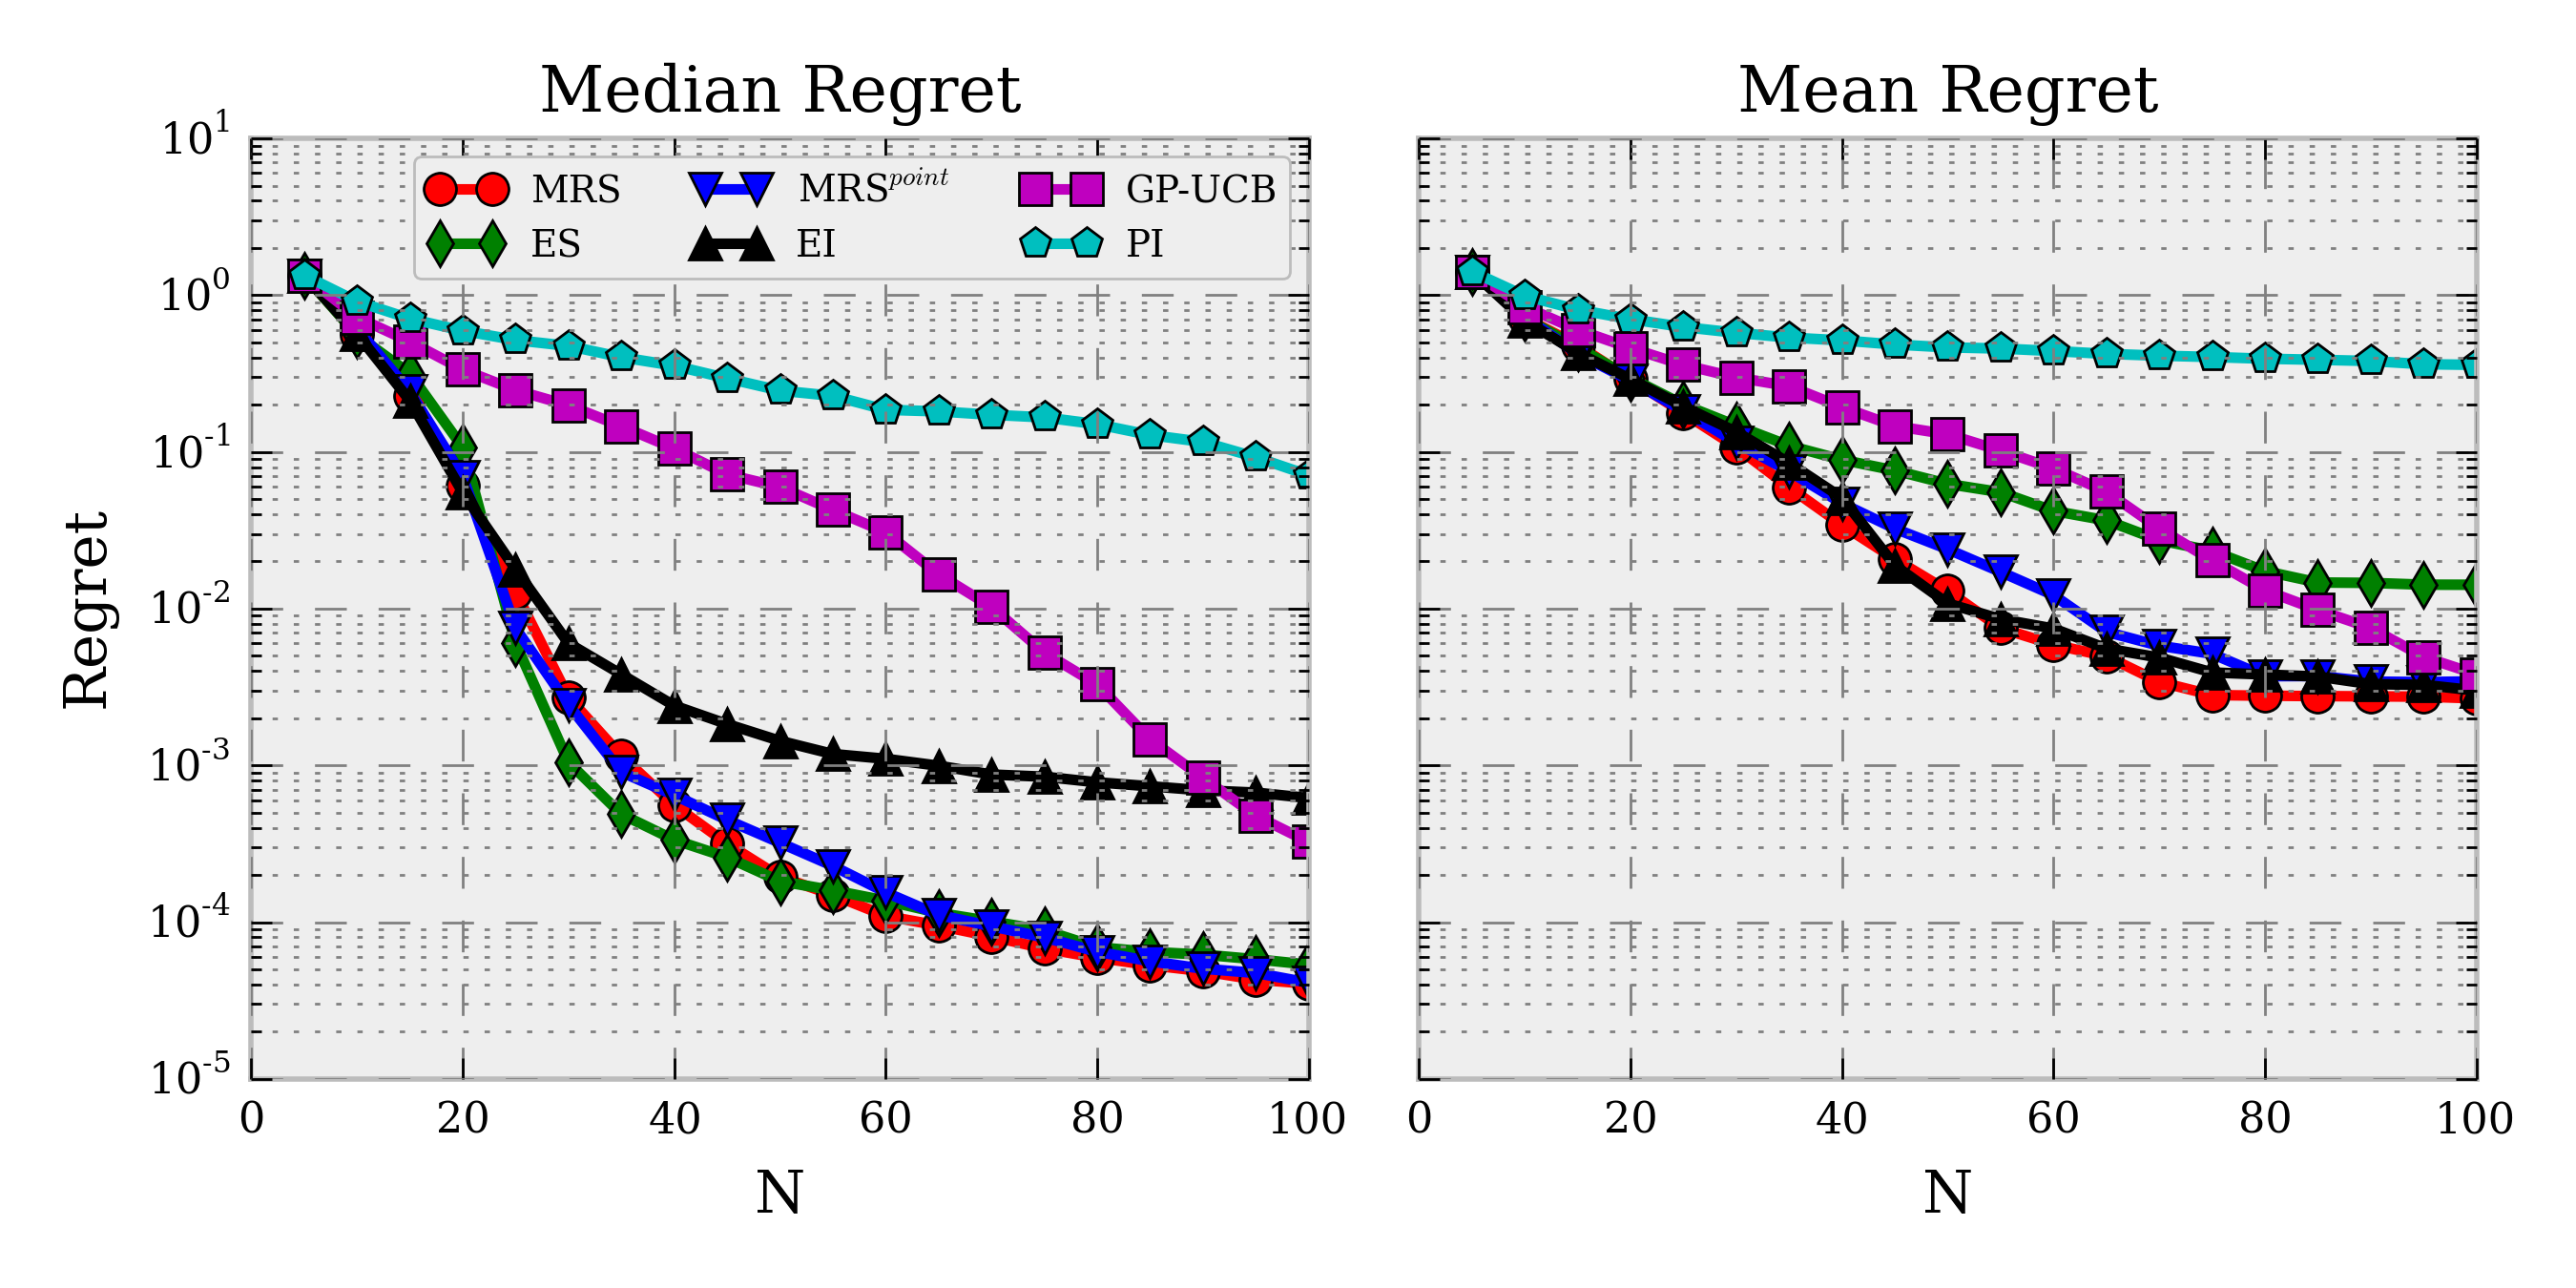
\includegraphics[width=.8\columnwidth]{../pics/empirical_comparison} \\
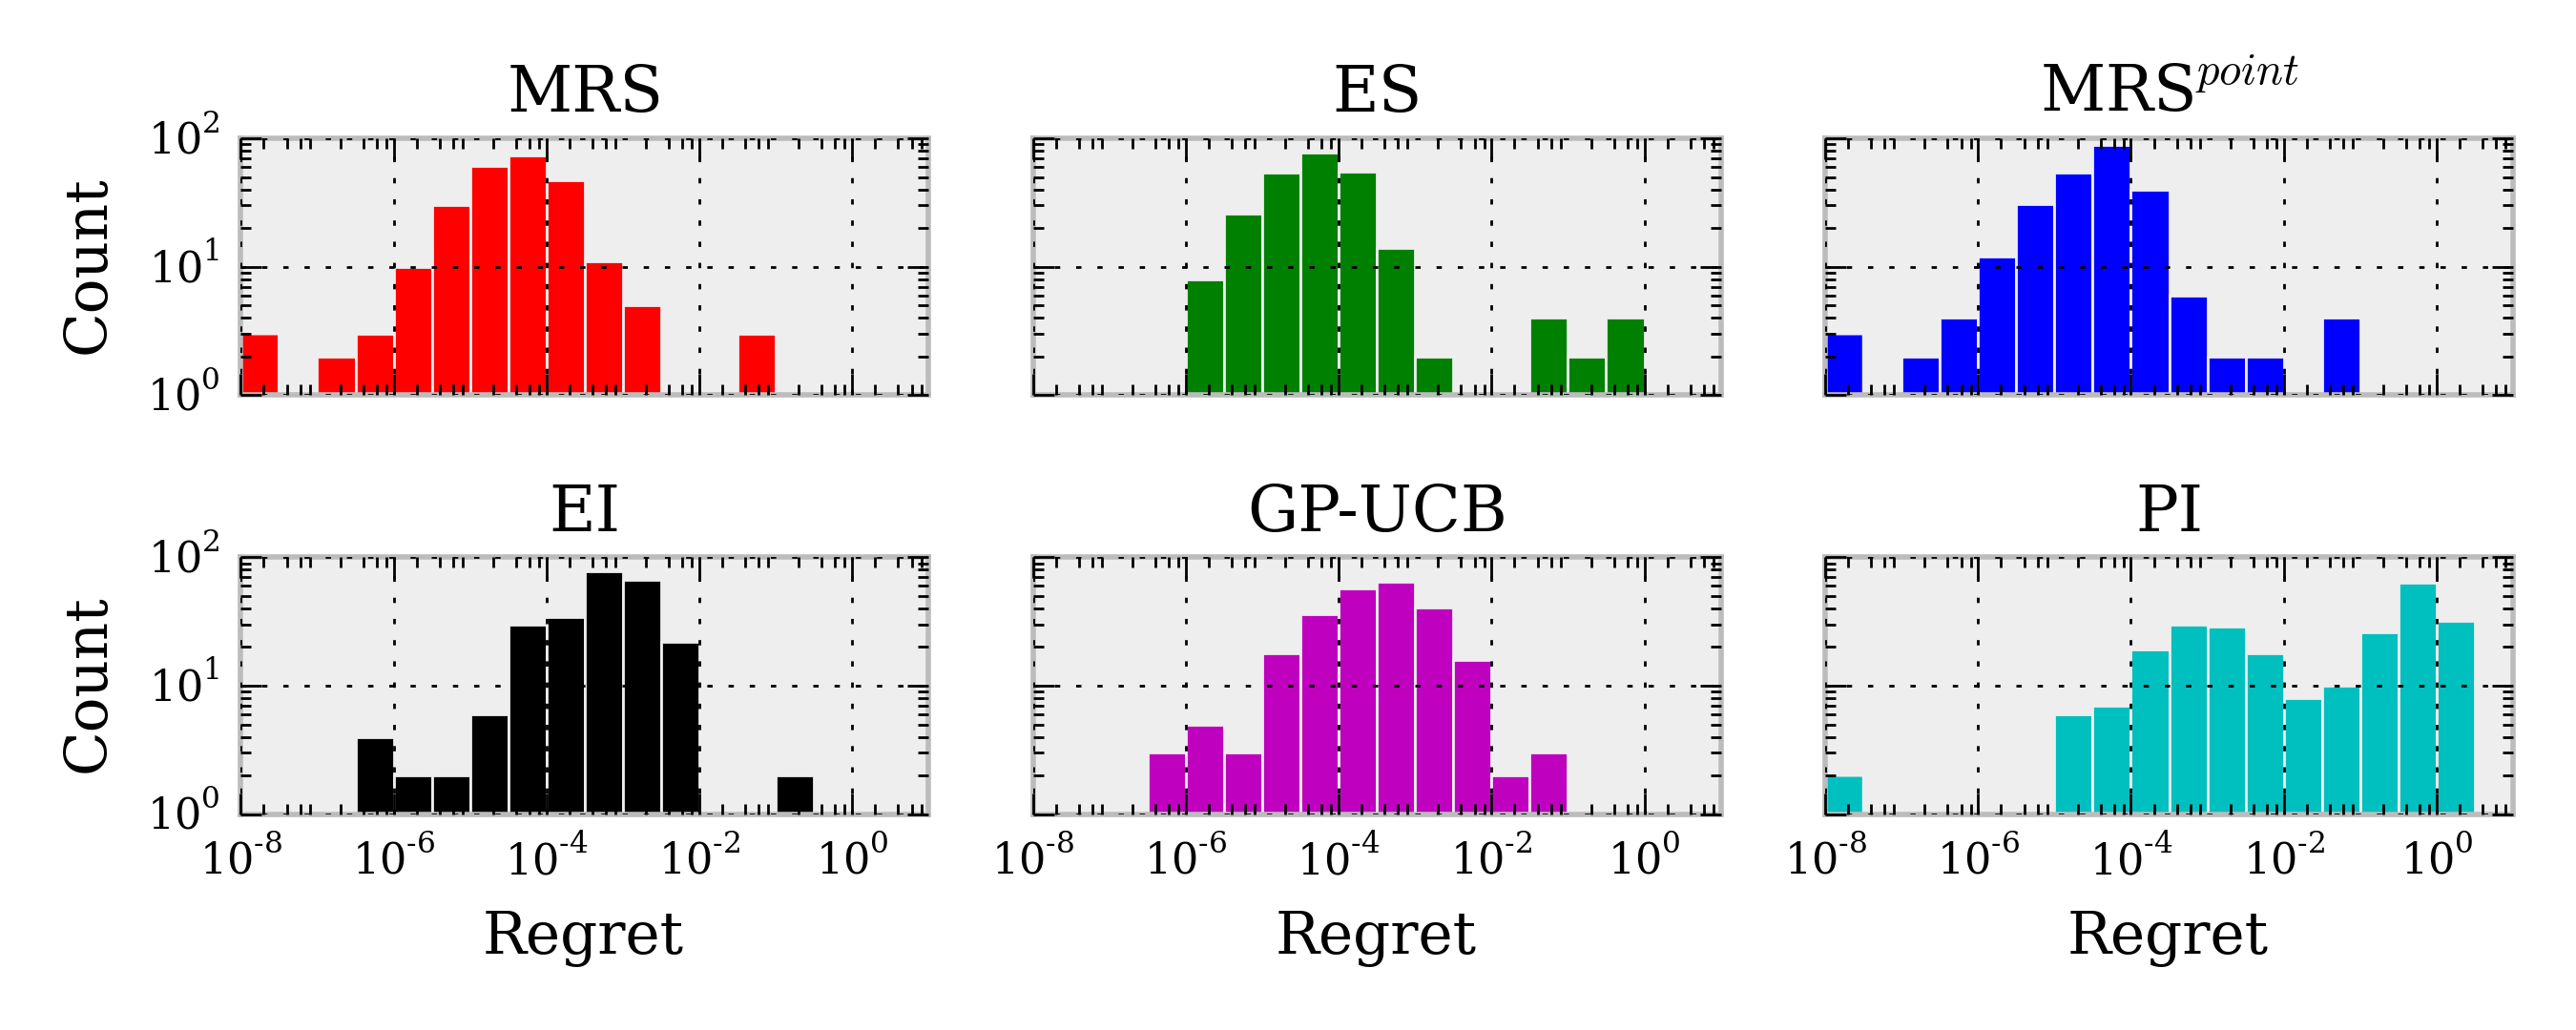
\includegraphics[width=.8\columnwidth]{../pics/hist}
\caption{\emph{No model mismatch:} Simple regret of the recommendation $\mathbf{\tilde x}_N$ after $N$ trials over $250$ repetitions for different acquisition functions.}
\label{fig:empirical_comparison}
\end{figure}


\begin{figure}
\centering
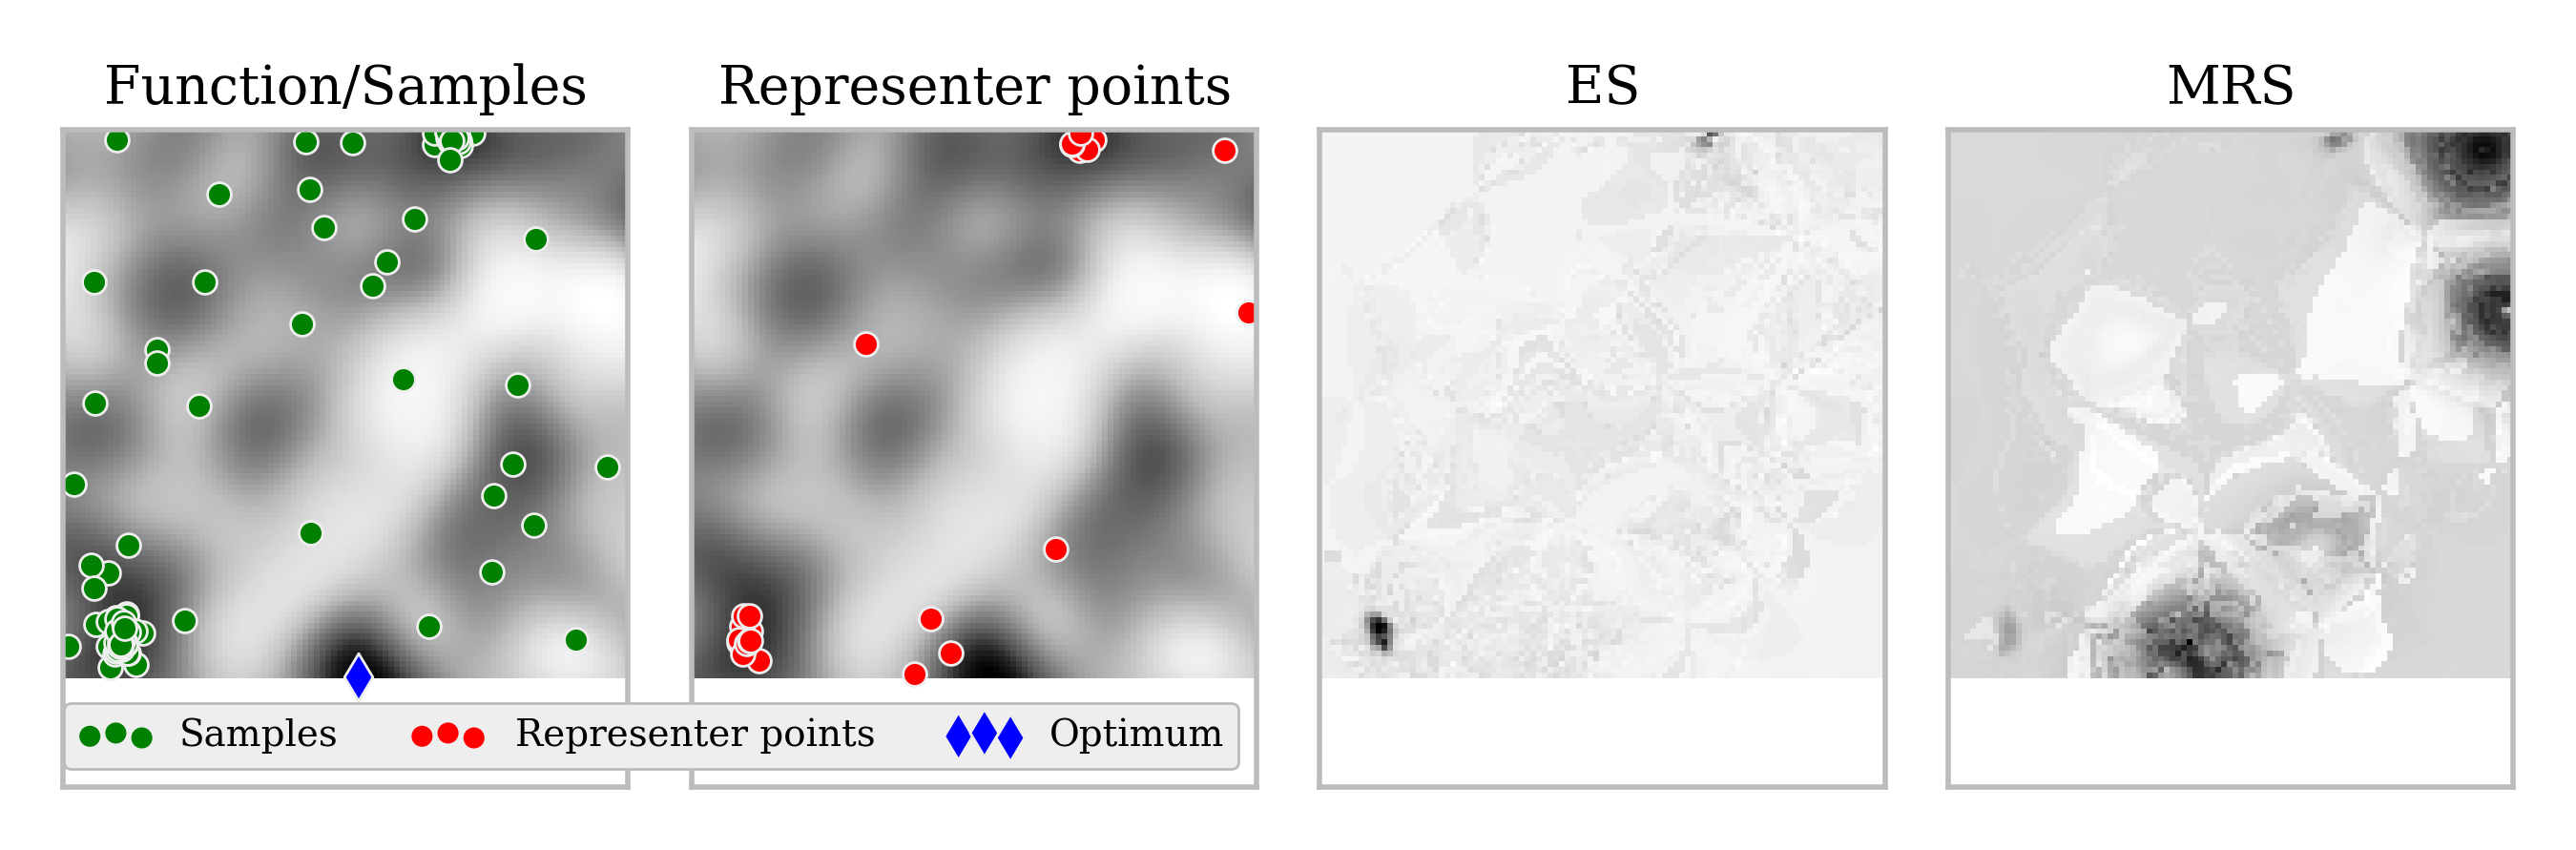
\includegraphics[width=.9\textwidth]{../pics/es_analysis}
\caption{Illustration of acquisition functions on a target function for
100 given samples and 25 representer points; darker areas correspond to larger values. ES focuses on sampling in areas with high density of $p^\star$ (many representer points), while MRS focuses on unexplored areas that are populated by representer points (non-zero $p^\star$).
}
\label{fig:es_analysis}
\end{figure}


\begin{figure}
\centering
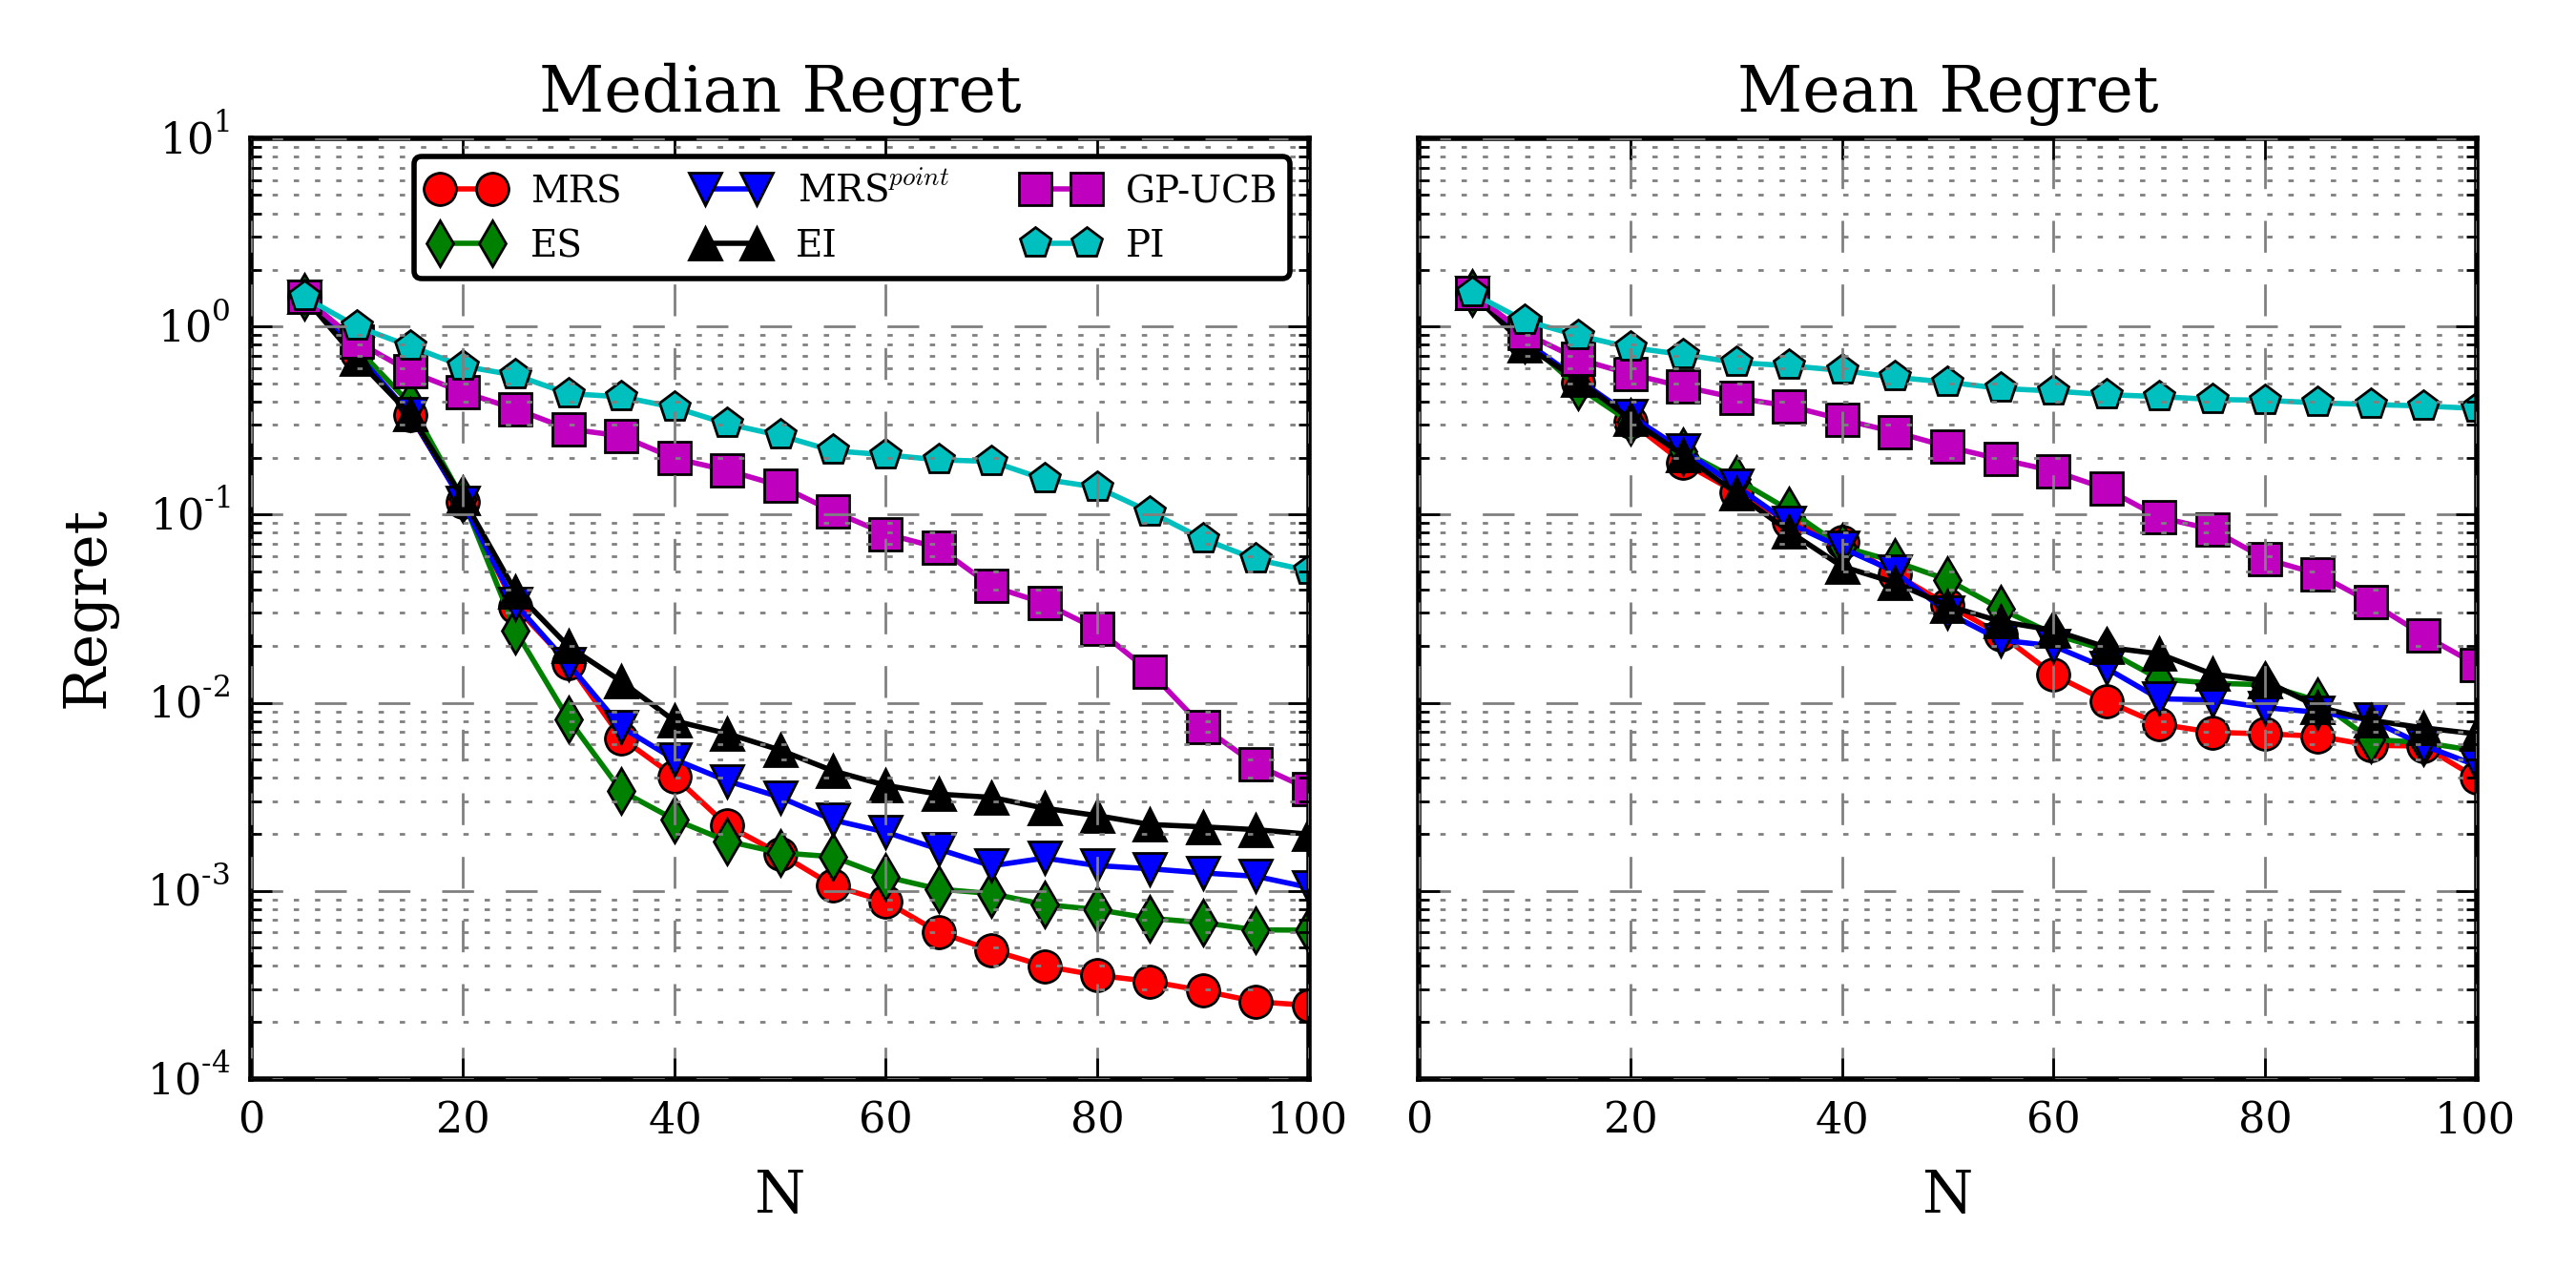
\includegraphics[width=.8\textwidth]{../pics/empirical_comparison_mm} \\
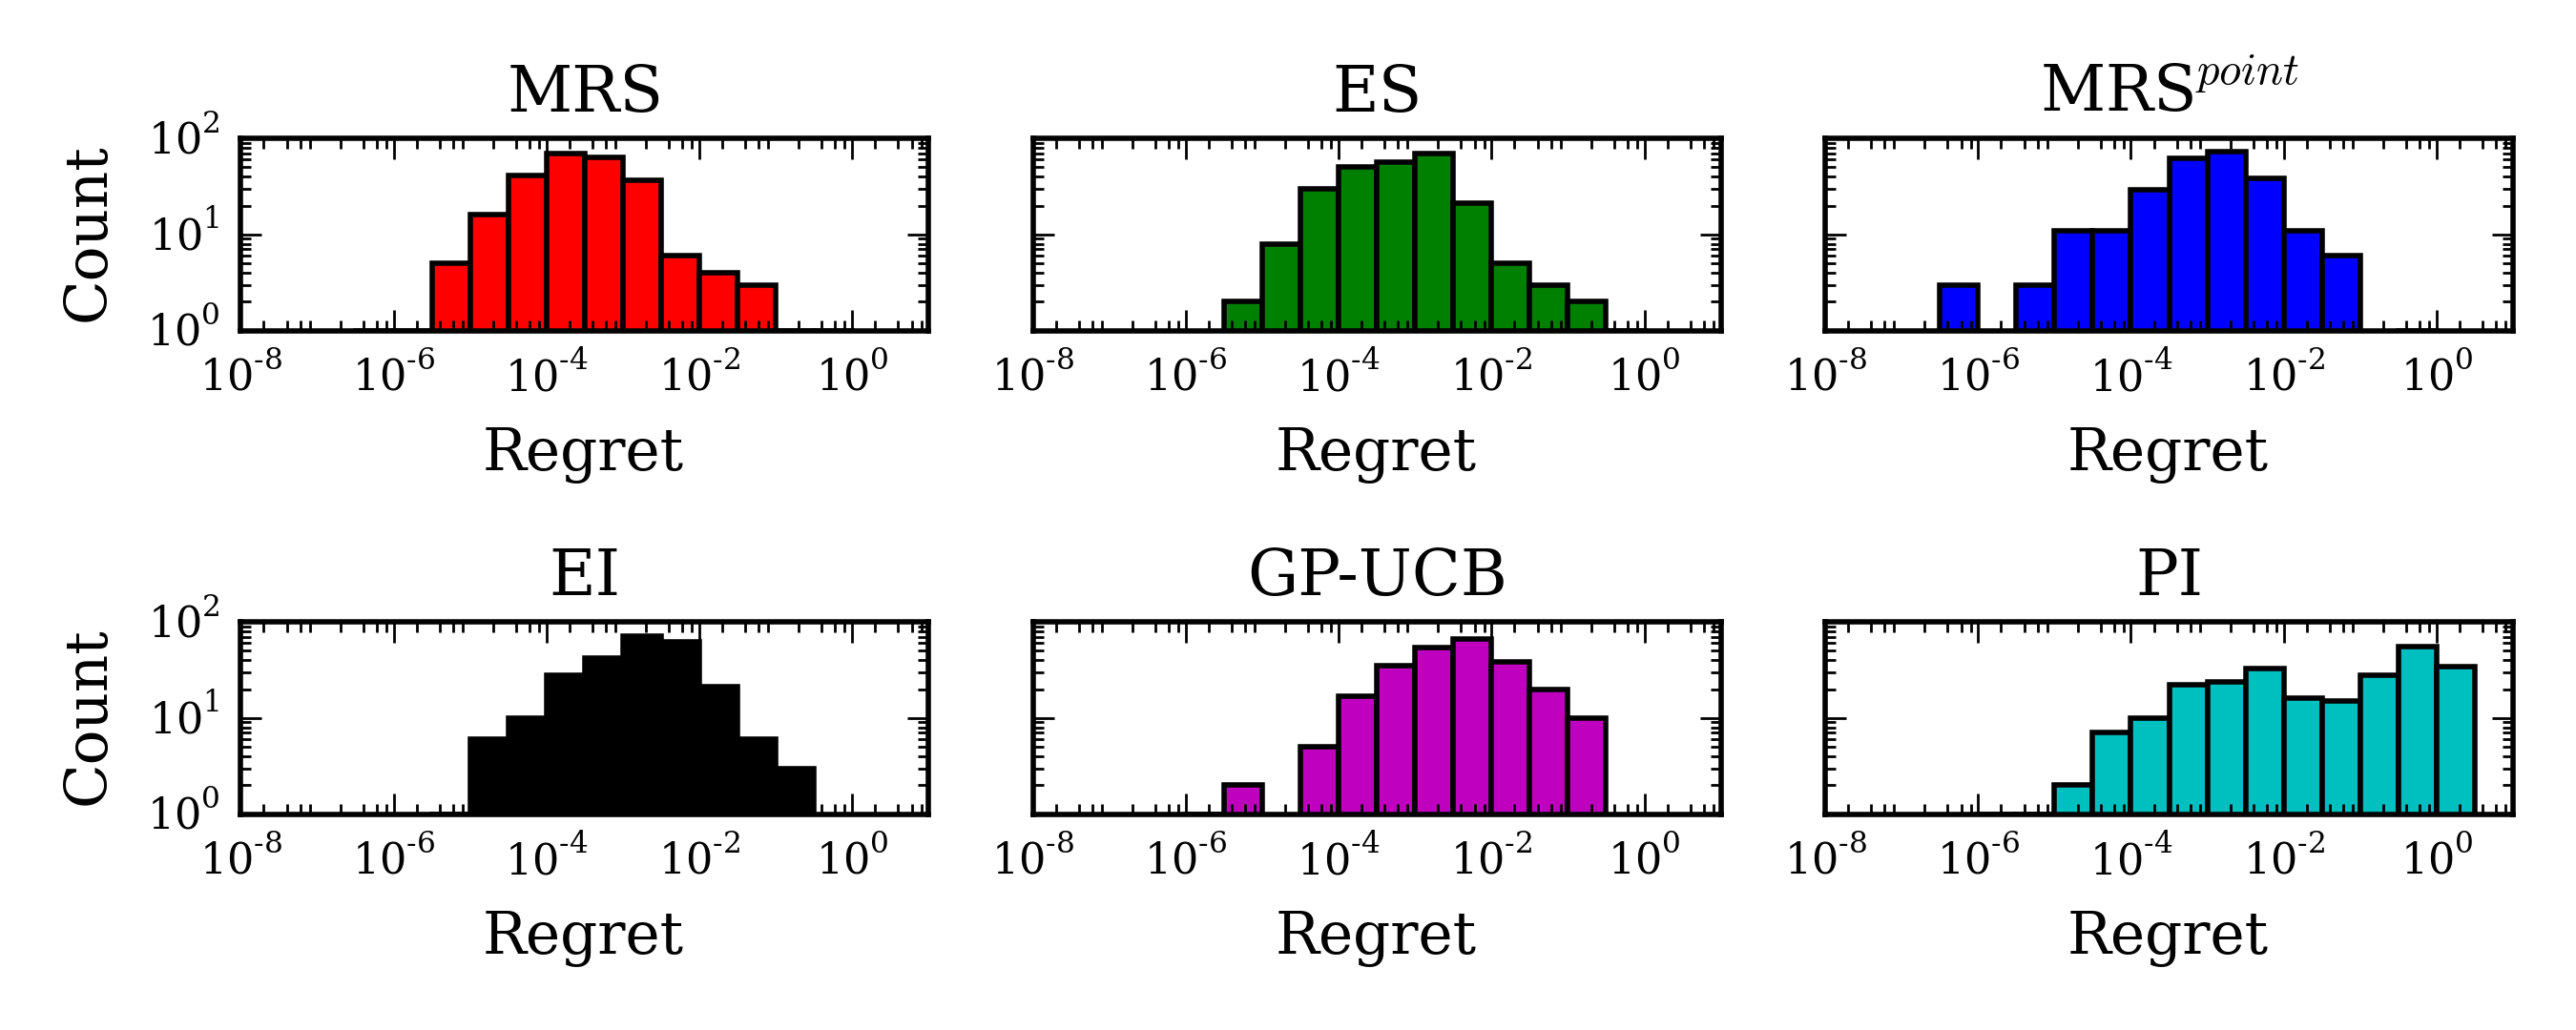
\includegraphics[width=.8\textwidth]{../pics/hist_mm}
\caption{\emph{Model mismatch:} Simple regret of the recommendation $\mathbf{\tilde x}_N$ after $N$ trials over $250$ repetitions for different acquisition functions.}
\label{fig:empirical_comparison_mm}
\end{figure}

\end{center}
\end{block}

\begin{block}{\blocktitle{Outlook}}
\begin{itemize}
 \item For multi-task learning and results on simulated robotic task: see paper
 \item Open questions: treatment of GP hyperparameters, more efficient approximation techniques for MRS, regret bounds for MRS?
\end{itemize}
\end{block}

\begin{block}{\blocktitle{References}}

\begin{multicols}{2}
{\scriptsize
\setbeamertemplate{bibliography item}[text]
\bibliographystyle{abbrv}
\bibliography{../literature}
}
\end{multicols}

\end{block}
